\section{Theoretische Grundlagen} \label{theo_grundl}

\subsection{Stromröhrentheorie}
Mithilfe der Stromröhrentheorie wird eine Energie- bzw. Leistungsbilanz des Luftmassenstromes \acs{mdot} in einer Stromröhre aufgestellt. Eine Stromröhre beschreibt einen Bilanzraum, welcher den Einfluss eines WEA-Rotors auf die Umgebung beinhaltet. Der Bilanzraum beginnt vor der WEA und endet hinter dieser. Die Ausbreitungsrichtung wird durch die Windrichtung vor dem Rotor bestimmt. \\
Durch eine erste vereinfachte Annahme, dass der Luftmassenstrom ungestört ist, wird eine mathematische Formel zur Berechnung der Windleistung \acs{PW} bestimmt. Anschließend erfolgt die Adaptierung durch die Annahme eines gestörten Luftmassenstromes. Dies führt zur Herleitung der entnommenen Rotorleistung \acs{PR} und des Leistungsbeiwertes \acs{cP}.

\subsubsection{Ungestörter Luftmassenstrom}

\paragraph{Stromröhrenmodell}\mbox{}\smallskip\\
Zur Modellierung der Stromröhre werden drei Querschnittsflächen (\acs{A1}, \acs{A2} und \acs{A3}) mit dem gleichen Flächeninhalt definiert. Die Ein- und Austrittsflächen (\acs{A1} und \acs{A3}) sind raumfest, d.h. diese ändern weder die Größe noch die Lage. Durch die Verbindung beider Flächen mithilfe von Stromlinien wird eine richtungsstationäre Mantelfläche aufgespannt (\autoref{fig:Bild2.1}).\\
\begin{figure}[H]
   \centering
   \fbox{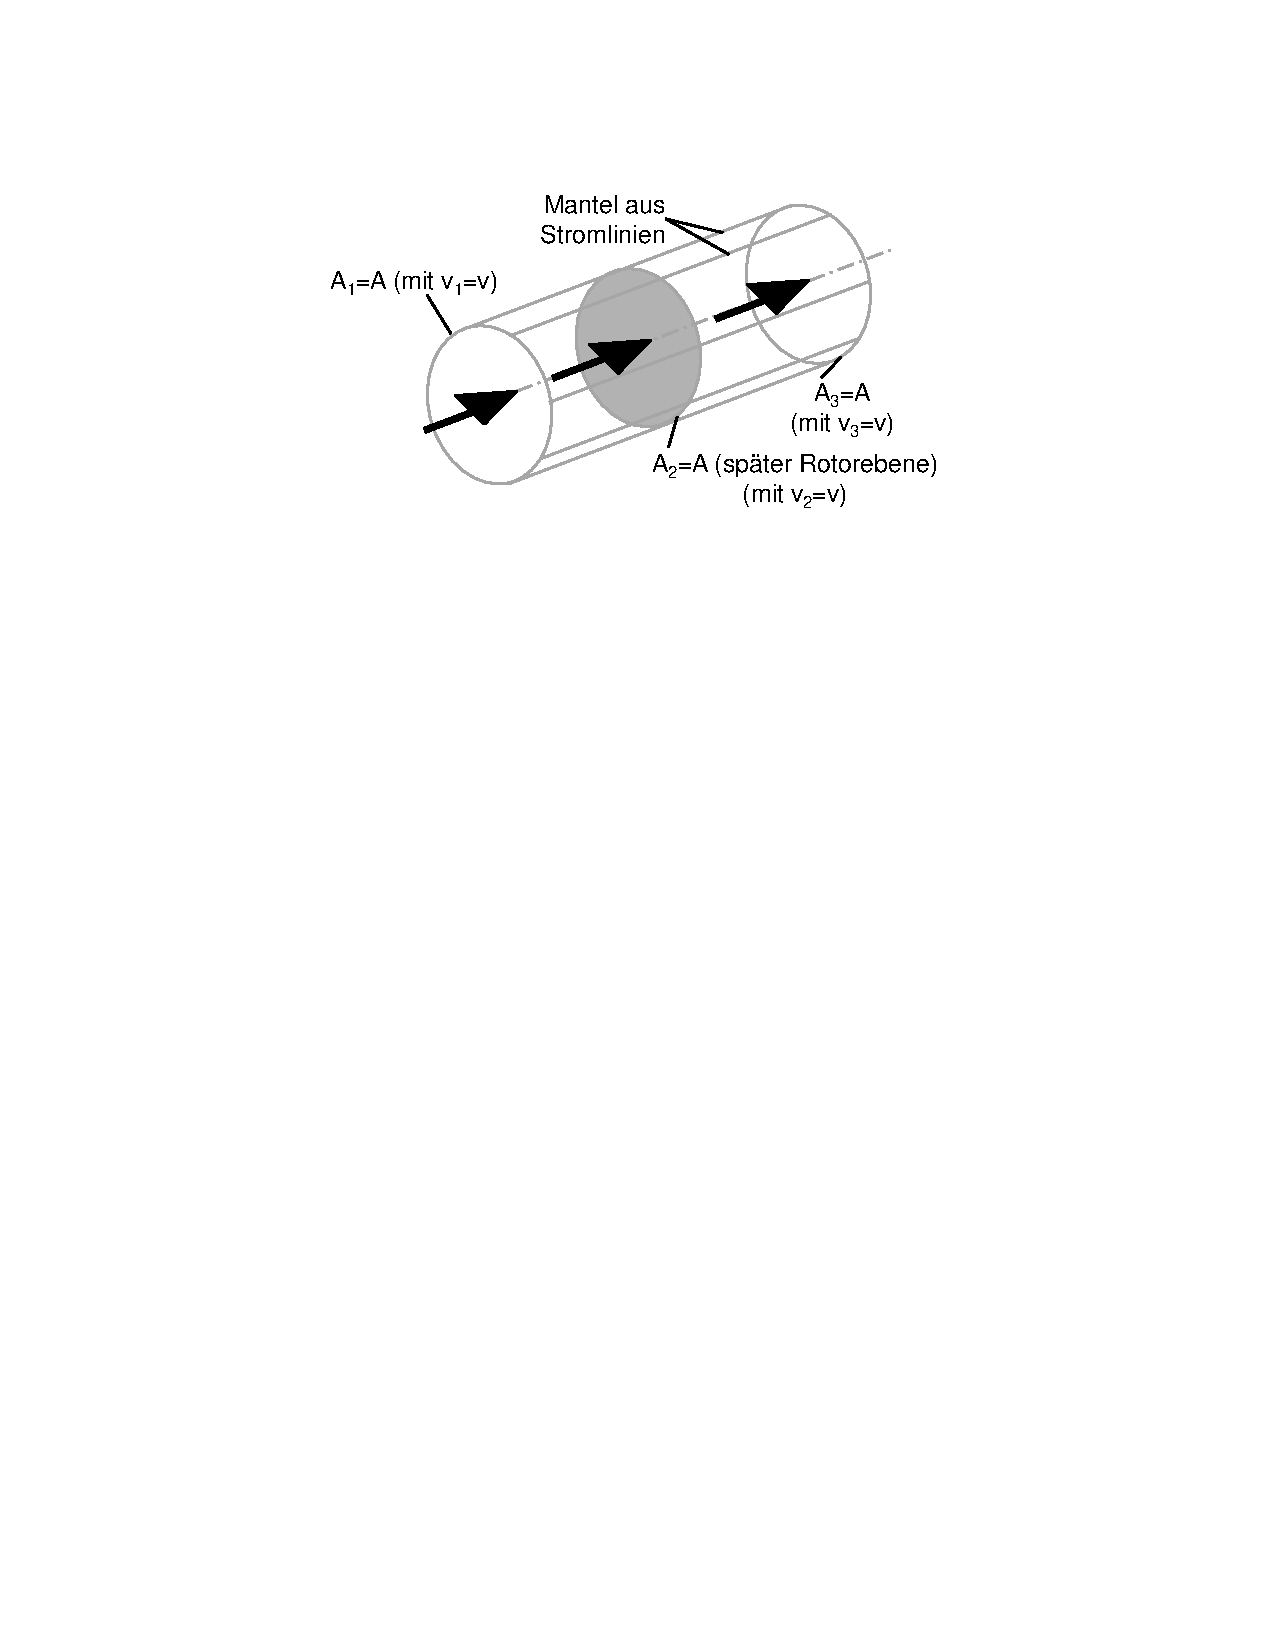
\includegraphics[width=0.5\textwidth]{Bilder/Kapitel 2/ungestörte_stromröhre.pdf}}
   \caption[Ungestörte Luftröhre]{Ungestörte Luftröhre}
   \label{fig:Bild2.1}
\end{figure}

Folgende weitere Annahmen werden getroffen:
\begin{itemize}
    \item konstante Querschnittsflächen: $\acs{Ai} = const.$
    \item stationäre gleichförmige Strömung: $\acs{vi}(t_{\mathrm{1}}) = \acs{vi}(t_{\mathrm{2}}) = \acs{vi} = const.$
    \item geringe Druckunterschiede: $\acs{rhoi} = const.$
    \item Index i = 1; 2; 3
\end{itemize}
\bigskip
Der ungestörte Luftmassenstrom folgt zu: 
\begin{equation} \label{eq:Gleichung2.1}
    \boxed{\acs{mdoti} = \acs{rhoi} \cdot \acs{vi} \cdot \acs{Ai} = const.}
\end{equation}

\paragraph{Windleistung \acs{PW}}\mbox{}\smallskip\\
Zur Berechnung der Windleistung \acs{PW} wird der ungestörten Luftmassenstroms (\autoref{eq:Gleichung2.1}) mit der Annahme, dass die Querschnittsflächen aus dem Rotoraußenradius \acs{R} berechnet werden (\autoref{eq:Gleichung2.2}) verwendet.
\begin{align}
    \acs{Ai} = \acs{pi}\cdot \acs{R}^2
    \label{eq:Gleichung2.2}
\end{align}
\newline
Die Windleistung folgt aus der zeitlichen Differentiation der kinetischen Windenergie \acs{EW} nach der Luftmasse \acs{m} und der Windgeschwindigkeit \acs{v}. 
\begin{align}
    \acs{EW} &= \frac{1}{2} \cdot \acs{mi} \cdot \acs{vi}^2 \nonumber \\
    \acs{PW} &= \frac{d}{dt}(\acs{EW}) \label{eq:Gleichung2.3} \\
    \acs{PW} &= \frac{1}{2} \cdot \acs{mdoti} \cdot \acs{vi}^2 + \frac{1}{2} \cdot \acs{mi} \cdot 2 \cdot \acs{vdoti}^2 \label{eq:Gleichung2.4}
\end{align}
\newline
Da eine stationäre Strömung vorliegt, ist die Änderung der Windgeschwindigkeit gleich Null ($\acs{vdoti} = 0$). Folglich wird die \autoref{eq:Gleichung2.4} vereinfacht.
\begin{align}
    \acs{PW} &= \frac{1}{2} \cdot \acs{mdoti} \cdot \acs{vi}^2 \label{eq:Gleichung2.5}
\end{align}
\newline
Durch das Einsetzen des ungestörten Luftmassenstromes aus \autoref{eq:Gleichung2.1} in die \autoref{eq:Gleichung2.5} resultiert die mathematische Formel zur Berechnung der zugefügten Windleistung \acs{PW}. Die Windgeschwindigkeit \acs{v1} und die Zwischenfläche \acs{A2} sind entscheidend. Die Luftdichte \acs{rho} wird wie o.g. als konstant angenommen.
\begin{align*}
    \acs{PW} &= \frac{1}{2} \cdot \acs{rho} \cdot \acs{v1} \cdot \acs{A2} \cdot \acs{v1}^2
\end{align*}
\begin{equation}\label{eq:Gleichung2.6}
    \boxed{\acs{PW} = \frac{1}{2} \cdot \acs{rho} \cdot \acs{A2} \cdot \acs{v1}^3} 
\end{equation}

\paragraph{Staukraft \acs{FST}}\mbox{}\smallskip\\
Zur Vorbereitung auf die Tragflügeltheorie wird die Formel zur Berechnung der Windleistung zu einem Produkt aus Staukraft \acs{FST} und ungestörter Windgeschwindigkeit \acs{v1} vereinfacht. Die Staukraft resultiert aus dem Produkt von Staudruck \acs{pST} und der Querschnittsfläche \acs{A2}.
\begin{align*}
    \acs{pST} = \frac{1}{2} \cdot \acs{rho} \cdot \acs{v1}^2 \\
    \acs{FST} = \acs{pST} \cdot \acs{A2}
\end{align*}
\begin{equation} \label{eq:Gleichung2.7}
    \boxed{\acs{PW} = \acs{FST} \cdot \acs{v1}}
\end{equation}

\subsubsection{Gestörter Luftmassenstrom}

\paragraph{Adaptierung des ungestörten Stromröhrenmodells}\mbox{}\smallskip\\
In der Realität liegt zwischen der Ein- und Austrittsfläche der Stromröhre ein Objekt (z.B. ein WEA-Rotor), welcher ein Strömungshindernis darstellt und den Luftmassenstrom verzögert (\autoref{fig:Bild2.2}). Die Verzögerung hat einen Abfall der Windgeschwindigkeiten $\acs{v2}$ und $\acs{v3}$ zur Folge.
\begin{align*}
    \acs{v1} > \acs{v2} > \acs{v3}
\end{align*}
\newline
Wird der ungestörte Luftmassenstrom mit gleichbleibender Windgeschwindigkeit $\acs{v2}$ und Querschnittfläche $\acs{A2}$ vorausgesetzt, muss die Querschnittsfläche $\acs{A1}$ verjüngt und die Fläche $\acs{A3}$ vergrößert werden, sodass weiterhin \autoref{eq:Gleichung2.1} gilt.
\begin{align*}
    \acs{A1} < \acs{A2} < \acs{A3}
\end{align*}
\begin{figure}[H]
   \centering
   \fbox{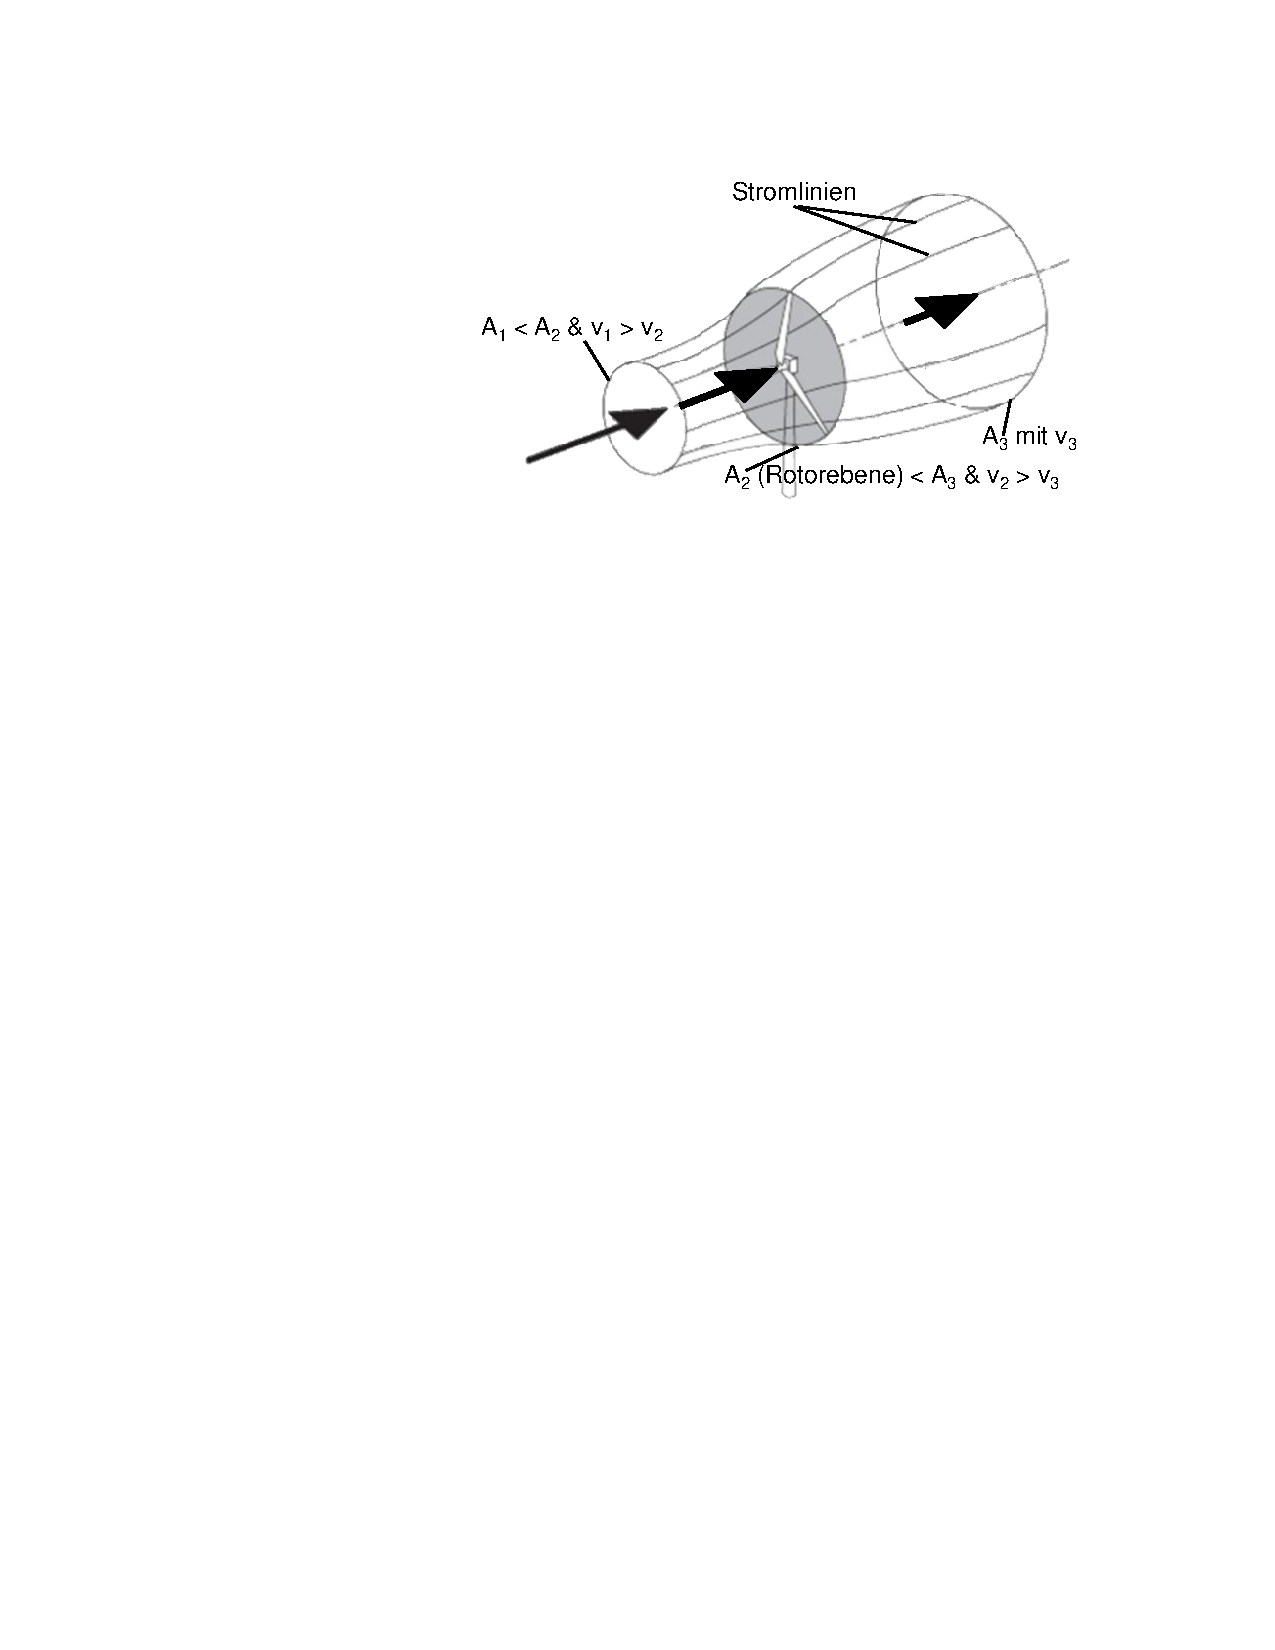
\includegraphics[width=0.5\textwidth]{Bilder/Kapitel 2/gestörte_stromröhre.pdf}}
   \caption[Gestörte Luftröhre]{Gestörte Luftröhre}
   \label{fig:Bild2.2}
\end{figure}

\paragraph{Drehzahlunabhängige Rotorleistung \acs{PR}}\mbox{}\smallskip\\
Die direkte Messung der Windgeschwindigkeit $\acs{v2}$ am Rotorblatt ist kaum möglich. Somit wird im ersten Ansatz die Rotorleistung $\acs{PR}$ mithilfe der \autoref{eq:Gleichung2.5} aus der Differenz der Windleistung vor dem Rotor und nach dem Rotor berechnet.
\begin{align*} \label{eq:Gleichung2.8}
    \acs{PR} = \acs{PW}(\acs{v1}) - \acs{PW}(\acs{v3})
\end{align*}
\begin{equation}\label{eq:Gleichung2.8}
    \boxed{\acs{PR} = \frac{1}{2} \cdot \acs{mdoti} \cdot (\acs{v1}^2 - \acs{v3}^2)}
\end{equation}

\paragraph{Einfluss der Rotordrehzahl \acs{nR}}\mbox{}\smallskip\\
Die entnommene Rotorleistung ist abhängig von der Windgeschwindigkeit $\acs{v2}$, der Rotordrehzahl \acs{nR} und aerodynamischen Effekten. Um die maximal mögliche Leistung für unterschiedliche Arbeitspunkte zu bestimmen, werden WEA-Kennfelder aufgenommen, welche im späteren Verlauf weiter definiert werden. Für eine erste Betrachtung über die Lage des Maximums werden zwei extreme Betriebspunkte festgelegt:
\begin{itemize}
    \item Rotorstillstand: $\acs{nR}$ = 0 $\rightarrow$ kaum Verzögerung
    \item Verblockung: $\acs{nR}$ >> 0 $\rightarrow$ nahezu Verstopfung
\end{itemize}

In beiden Fällen ist die entnommene Rotorleistung annähernd Null. Aus den Grenzfällen wird geschlussfolgert, dass das Maximum der Rotorleistung zwischen diesen Punkten liegen muss.\\
Aus dem Froude-Rankineschen Theorem geht hervor, dass die Windgeschwindigkeit des Rotors $\acs{v2}$ den Mittelwert der ungestörten Windgeschwindigkeit $\acs{v1}$ und der reduzierten Windgeschwindigkeit $\acs{v3}$ darstellt. Somit gilt:
\begin{equation}\label{eq:Gleichung2.9}
    \boxed{\acs{v2} = \frac{\acs{v1} + \acs{v3}}{2}}
\end{equation}
\newline
Der resultierende Luftmassenstrom gemäß \autoref{eq:Gleichung2.5} folgt zu:
\begin{align*}
    \acs{mdot} = \acs{rho} \cdot \acs{v2} \cdot \acs{A2}
\end{align*}
\begin{equation}\label{eq:Gleichung2.10}
    \boxed{\acs{mdot} = \acs{rho} \cdot \frac{\acs{v1} + \acs{v3}}{2} \cdot \acs{A2}}
\end{equation}
\newline
Durch das Einsetzen der Zusammenhänge aus \autoref{eq:Gleichung2.8} in \autoref{eq:Gleichung2.10} folgt die Gleichung zur Berechnung der Rotorleistung $\acs{PR}$ in Abhängigkeit der Rotordrehzahl $\acs{nR}$.
\begin{align*}
    \acs{PR} &= \frac{1}{2} \cdot \acs{rho} \cdot \frac{\acs{v1} + \acs{v3}}{2} \cdot \acs{A2} \cdot (\acs{v1}^2 - \acs{v3}^2) \\
    \acs{PR} &= \frac{1}{2} \cdot \acs{rho} \cdot \acs{A2} \cdot \frac{1}{2} \cdot \acs{v1} \cdot (1 + \frac{\acs{v3}}{\acs{v1}}) \cdot \acs{v1}^2 \cdot (1 - \frac{\acs{v3}^2}{\acs{v1}^2})
\end{align*}
\newline
Wird nun der Term $(\frac{1}{2} \cdot \acs{rho} \cdot \acs{v1} \cdot \acs{A2} \cdot \acs{v1}^2)$ durch $\acs{PW}$ aus \autoref{eq:Gleichung2.6} ersetzt, resultiert:
\begin{equation}\label{eq:Gleichung2.11}
    \boxed{\acs{PR} = \acs{PW} \cdot \frac{1}{2} \cdot (1 + \frac{\acs{v3}}{\acs{v1}}) \cdot (1 - \frac{\acs{v3}^2}{\acs{v1}^2})}
\end{equation}

\paragraph{Leistungsbeiwert \acs{cP}}\mbox{}\smallskip\\
Die \autoref{eq:Gleichung2.11} wird weiter zu einem Produkt aus der Windleistung $\acs{PW}$ und einem dimensionslosen Leistungsbeiwert $\acs{cP}$ zusammengefasst. Der Leistungsbeiwert nimmt nur Werte zwischen Null und Eins an und beschreibt das Verhältnis von entnommener Rotorleistung $\acs{PR}$ zu zugefügter Windleistung $\acs{PW}$.
\begin{align*}
    \acs{cP} = \frac{1}{2} \cdot (1 + \frac{\acs{v3}}{\acs{v1}}) \cdot (1 - \frac{\acs{v3}^2}{\acs{v1}^2})
\end{align*}
\begin{equation}\label{eq:Gleichung2.12}
    \boxed{\acs{PR} = \acs{PW} \cdot \acs{cP}}
\end{equation}
\begin{equation}\label{eq:Gleichung2.13}
    \boxed{\acs{cP} = \frac{\acs{PR}}{\acs{PW}}}
\end{equation}
\newline
Ist der Leistungsbeiwert gleich Eins, entnimmt die WEA 100\% der Windleistung. Dies ist in der Realität u.a. aufgrund von aerodynamischen Effekten nicht möglich. Bei einer optimalen Verzögerung wird ein Wert von ca. 59\% ($\frac{16}{27}$) erreicht, welcher als Betzscher Leistungsbeiwert ($\acs{cPmax}$) bezeichnet wird. Dieser Wert wird ausschließlich bei folgender Konstellation ausgehend von der Windgeschwindigkeit $\acs{v1}$ erreicht. Diese Annahme ist jedoch hypothetisch, d.h. in Realität liegt der maximale Leistungsbeiwert bei ca. 45 bis 48\%.
\begin{itemize}
    \item $\acs{v2} = \frac{2}{3} \cdot \acs{v1}$
    \item $\acs{v3} = \frac{1}{3} \cdot \acs{v1}$
\end{itemize}
Weichen die Windgeschwindigkeiten am Rotor und hinter der WEA von den o.g. Faktoren ab, ist das Verhältnis von entnommener zu zugefügter Leistung geringer als der Betzsche Leistungsbeiwert.

\subsection{Tragflügeltheorie}

\subsubsection{Auftrieb und Widerstand eines Tragflügels}
Wird ein Tragflügel von einem Wind der Geschwindigkeit $\acs{v}$ erfasst, entsteht eine resultierende Geschwindigkeit $\acs{c}$ (Anströmgeschwindigkeit) (\autoref{fig:Bild2.3}), welche über die Wurzel der quadratischen Summe aus Windgeschwindigkeit $\acs{v}$ und der relativen Bewegungsgeschwindigkeit $\acs{u'}$ berechnet wird (\autoref{eq:Gleichung2.14}). Die relative Bewegungsgeschwindigkeit \acs{u'} folgt aus der Negation der quer zur Windgeschwindigkeit stehenden Bewegungsgeschwindigkeit \acs{u}.
\begin{align} \label{eq:Gleichung2.14}
    \acs{c} = \sqrt{\acs{v}^2 + (\acs{u'})^2}
\end{align}
\begin{figure}[H]
   \centering
   \fbox{\includegraphics[width=0.34\textwidth]{Bilder/Kapitel 2/auftrieb_widerstand_tragflügel.pdf}}
   \caption[Anströmverhältnisse eines Tragflügels]{Anströmverhältnisse eines Tragflügels}
   \label{fig:Bild2.3}
\end{figure}

Die Anströmgeschwindigkeit ist über die Tragflügellänge konstant. Durch die Luftanströmung werden Luftpartikel an der oberen Tragflügelseite beschleunigt und an der unteren Tragflügelseite abgebremst. Dadurch entstehen eine Saugseite (beschleunigte Luftpartikel) und eine Druckseite (gebremste Luftpartikel). Die unterschiedlichen Strömungsgeschwindigkeiten führen zu einem Druckunterschied zwischen der oberen und unteren Tragflügelseite. Der Überdruck unter dem Tragflügel führt zu einer Auftriebskraft \acs{FA}, wohingegen der Unterdruck auf der Oberseite eine Widerstandkraft \acs{FW} hervorruft (\autoref{fig:Bild2.4}).
\begin{figure}[H]
   \centering
   \fbox{\includegraphics[width=0.39\textwidth]{Bilder/Kapitel 2/druckverhältnisse.pdf}}
   \caption[Saug- und Druckseite]{Saug- und Druckseite}
   \label{fig:Bild2.4}
\end{figure}
\newpage
\paragraph{Kräfte}\mbox{}\smallskip\\
Durch die Abgrenzung von Saug- und Druckseite durch eine Profilsehne entsteht ein Anstellwinkel \acs{alpha} zwischen der Profilsehne und des Vektors der Anströmgeschwindigkeit \acs{c}. Die Widerstandkraft verläuft in Richtung der Anströmgeschwindigkeit, wohingegen die Auftriebskraft senkrecht zu dieser steht (\autoref{fig:Bild2.5}). Aus den Kenntnissen über die Tiefe \acs{tflug} und Breite \acs{bflug} eines Tragflügels werden die Auftriebs- und Widerstandkraft nach \autoref{eq:Gleichung2.15} und \autoref{eq:Gleichung2.16} berechnet.
\begin{align}
    \acs{FA} = \acs{cA}(\acs{alpha}) \cdot \frac{1}{2} \cdot \acs{rho} \cdot \acs{c}^2 \cdot (\acs{tflug} \cdot \acs{bflug}) \label{eq:Gleichung2.15} \\
    \acs{FW} = \acs{cW}(\acs{alpha}) \cdot \frac{1}{2} \cdot \acs{rho} \cdot \acs{c}^2 \cdot (\acs{tflug} \cdot \acs{bflug}) \label{eq:Gleichung2.16}
\end{align}
\begin{figure}[H]
   \centering
   \fbox{\includegraphics[width=0.6\textwidth]{Bilder/Kapitel 2/kräfte.pdf}}
   \caption[Auftriebs- und Widerstandskraft]{Auftriebs- und Widerstandskraft}
   \label{fig:Bild2.5}
\end{figure}

\paragraph{Beiwerte}\mbox{}\smallskip\\
Die Faktoren \acs{cA} und \acs{cW} stellen den Auftriebs- und Widerstandsbeiwert dar und hängen vom Anstellwinkel \acs{alpha} ab. Die jeweiligen Werte werden messtechnisch ermitteln und sind für jede Tragflügelkontur unterschiedlich (\autoref{fig:Bild2.6}).
\begin{figure}[H]
   \centering
   \fbox{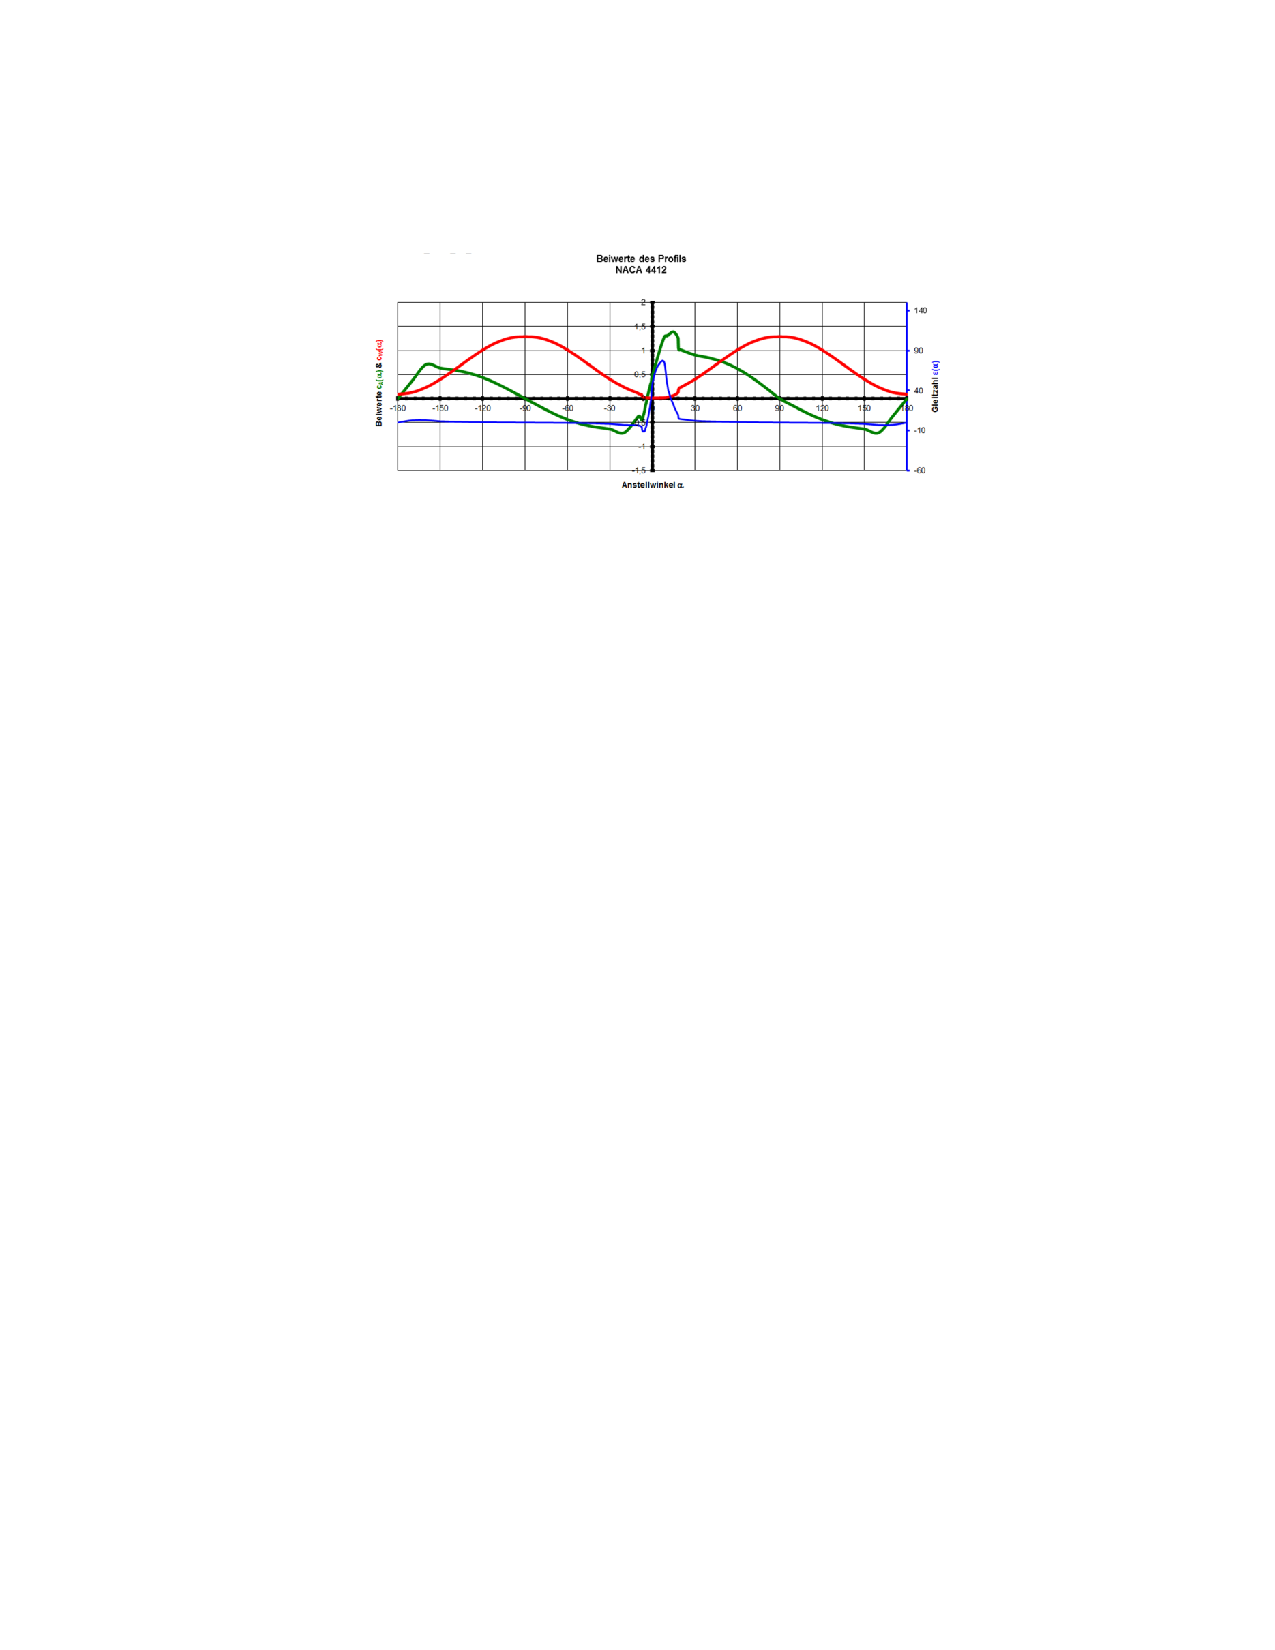
\includegraphics[width=0.5\textwidth]{Bilder/Kapitel 2/beiwerte.pdf}}
   \caption[Beispielverlauf der Beiwerte]{Beispielverlauf der Beiwerte}
   \label{fig:Bild2.6}
\end{figure}
\newpage
Wird der Quotient aus Antriebskraft \acs{FA} und Widerstandskraft \acs{FW} gebildet, folgt die Gleitzahl \acs{eps}. Diese Verhältnis wird optimal, wenn im Verhältnis zum Widerstand ein maximaler Auftrieb erzeugt wird. Daraus resultiert ein optimaler Anstellwinkel \acs{alphaopt}.
\begin{align}
    \frac{\acs{FA}}{\acs{FW}} &= \frac{\acs{cA}(\acs{alpha}) \cdot \frac{1}{2} \cdot \acs{rho} \cdot \acs{c}^2 \cdot (\acs{tflug} \cdot \acs{bflug})}{\acs{cW}(\acs{alpha}) \cdot \frac{1}{2} \cdot \acs{rho} \cdot \acs{c}^2 \cdot (\acs{tflug} \cdot \acs{bflug})} \nonumber \\
    \frac{\acs{FA}}{\acs{FW}} &= \frac{\acs{cA}(\alpha)}{\acs{cW}(\alpha)} \label{eq:Gleichung2.17}
\end{align}
\begin{equation} \label{eq:Gleichung2.18}
    \boxed{\acs{eps}(\acs{alpha}) = \frac{\acs{FA}}{\acs{FW}}}
\end{equation}
\newline
Wird ein blattprofilspezifischer Wert des Anstellwinkels überschritten, folgt ein Strömungsabriss, d.h. die Luftpartikel folgen nicht länger der Tragflügelkontur.

\subsubsection{Anströmverhältnisse am Rotorblatt}

\paragraph{Anströmungs- und Umfangsgeschwindigkeit}\mbox{}\smallskip\\
Basierend auf \autoref{eq:Gleichung2.14} wird die Anströmungsgeschwindigkeit $\acs{c}\left(\acs{R}, \acs{nR}\right)$ aus der Wurzel der quadratischen Summe von der Windgeschwindigkeit \acs{v2} in der Rotorebene und der Umfangsgeschwindigkeit $\acs{u}\left(\acs{R}, \acs{nR}\right)$ infolge der Rotordrehung berechnet (\autoref{eq:Gleichung2.19}) (\autoref{fig:Bild2.7}).
\begin{equation} \label{eq:Gleichung2.19}
    \boxed{\acs{c}\left(\acs{R}, \acs{nR}\right) = \sqrt{\acs{v2}^2 + \acs{u}(\acs{R}, \acs{nR})^2}}
\end{equation}
\begin{figure}[H]
   \centering
   \fbox{\includegraphics[width=0.6\textwidth]{Bilder/Kapitel 2/anströmungs_umfangsgeschwindigkeit.pdf}}
   \caption[Antrömverhältnisse eines Rotorblattes]{Anströmverhältnisse eines Rotorblattes}
   \label{fig:Bild2.7}
\end{figure}

Die Umfangsgeschwindigkeit \acs{u} des Rotors ist abhängig von der Rotordrehzahl \acs{nR} und dem Rotoraußenradius \acs{R} (\autoref{eq:Gleichung2.20}). Mit steigendem Radius zur Blattspitze nimmt die Umfangsgeschwindigkeit und somit auch die Anströmgeschwindigkeit zu.
\begin{equation} \label{eq:Gleichung2.20}
    \boxed{\acs{u}(\acs{R}, \acs{nR}) = \acs{omegaR} \cdot \acs{R} = 2 \cdot \acs{pi} \cdot \acs{nR} \cdot \acs{R}}
\end{equation}

\paragraph{Schnelllaufzahl}\mbox{}\smallskip\\
Zur aerodynamischen Auslegung der Rotorblätter ist die Kenntnis über das Verhältnis von Blattspitzengeschwindigkeit $\acs{u}\left(\acs{R}, \acs{nR}\right)$ zur ungestörten Windgeschwindigkeit \acs{v1} wichtig. Dieses Verhältnis wird als Schnelllaufzahl \acs{lambda} deklariert.
\begin{equation} \label{eq:Gleichung2.21}
    \boxed{\acs{lambda}\left(\acs{R}, \acs{nR}\right) = \frac{\acs{u}\left(\acs{R}, \acs{nR}\right)}{\acs{v1}} = \frac{\acs{omegaR}\left(\acs{nR}\right) \cdot \acs{R}}{\acs{v1}}}
\end{equation}

\paragraph{Anstell- und Anströmwinkel}\mbox{}\smallskip\\
Der Anstellwinkel $\acs{alpha}\left(\acs{R}\right)$ hängt vom Tragflügelprofil ab und repräsentiert den Winkel zwischen der Anströmgeschwindigkeit $\acs{c}\left(\acs{R}, \acs{nR}\right)$ und der Profilsehne, welche die Trennlinie zwischen der Druck- und Saugseite darstellt (\autoref{fig:Bild2.8}).
\begin{figure}[H]
   \centering
   \fbox{\includegraphics[width=0.6\textwidth]{Bilder/Kapitel 2/anstell_anströmwinkel.pdf}}
   \caption[Anstell- und Anströmwinkel]{Anstell- und Anströmwinkel}
   \label{fig:Bild2.8}
\end{figure}

Der Anströmwinkel $\acs{gamma}\left(\acs{R}, \acs{nR}\right)$ hängt von der Windgeschwindigkeit \acs{v2} und der Umfangsgeschwindigkeit $\acs{u}\left(\acs{R}, \acs{nR}\right)$ ab. Sind beide Größen bekannt, resultiert der Anströmwinkel aus folgender \autoref{eq:Gleichung2.22}.
\begin{equation} \label{eq:Gleichung2.22}
	\boxed{\acs{gamma}\left(\acs{R}, \acs{nR}\right) = \arctan\left(\frac{\acs{v2}}{\acs{u}\left(\acs{R}, \acs{nR}\right)}\right)}
\end{equation}
\newline
Die eben aufgeführte Gleichung hängt ebenso wie die Anströmgeschwindigkeit \acs{c} nur von der Windgeschwindigkeit \acs{v2} in der Rotorebene und der Umfangsgeschwindigkeit $\acs{u}\left(\acs{R}, \acs{nR}\right)$ ab. Somit hängt die Anströmgeschwindigkeit \acs{gamma} direkt vom Anströmwinkel \acs{alpha} ab. Es gilt:
\begin{equation} \label{eq:Gleichung2.23}
	\boxed{\acs{c}\left(\acs{R}, \acs{nR}\right) = \acs{c}\left(\acs{gamma}(\acs{R}, \acs{nR})\right)}
\end{equation}

\paragraph{Bauwinkel}\mbox{}\smallskip\\
Der Bauwinkel $\acs{beta}\left(\acs{R}, \acs{nR}\right)$ wird beim Entwurf eines neuen Rotorblattes festgelegt und liegt zwischen der Rotorebene und der Profilsehne (\autoref{fig:Bild2.9}). Auf Grundlage dessen resultiert ein optimales Anströmverhältnis aus Antriebskraft $\acs{FA}\left(\acs{alpha}\left(\acs{R}, \acs{nR}\right)\right)$ zu Widerstandskraft $\acs{FW}\left(\acs{alpha}\left(\acs{R}, \acs{nR}\right)\right)$. Der Anstellwinkel $\acs{alpha}\left(\acs{R}, \acs{nR}\right)$ liegt genau im Optimum $\acs{alphaopt}\left(\acs{R}, \acs{nR}\right)$. Durch den Einbauwinkel kann der Anströmwinkel $\acs{gamma}\left(\acs{R}, \acs{nR}\right)$ aus der Summe von Anstellwinkel $\acs{alpha}\left(\acs{R}, \acs{nR}\right)$ und Bauwinkel $\acs{beta}\left(\acs{R}, \acs{nR}\right)$ berechnet werden (\autoref{eq:Gleichung2.24}).
\begin{align} \label{eq:Gleichung2.24}
	\acs{gamma}\left(\acs{R}, \acs{nR}\right) = \acs{alpha}\left(\acs{R}, \acs{nR}\right) + \acs{beta}\left(\acs{R}, \acs{nR}\right)
\end{align}
\begin{figure}[H]
   \centering
   \fbox{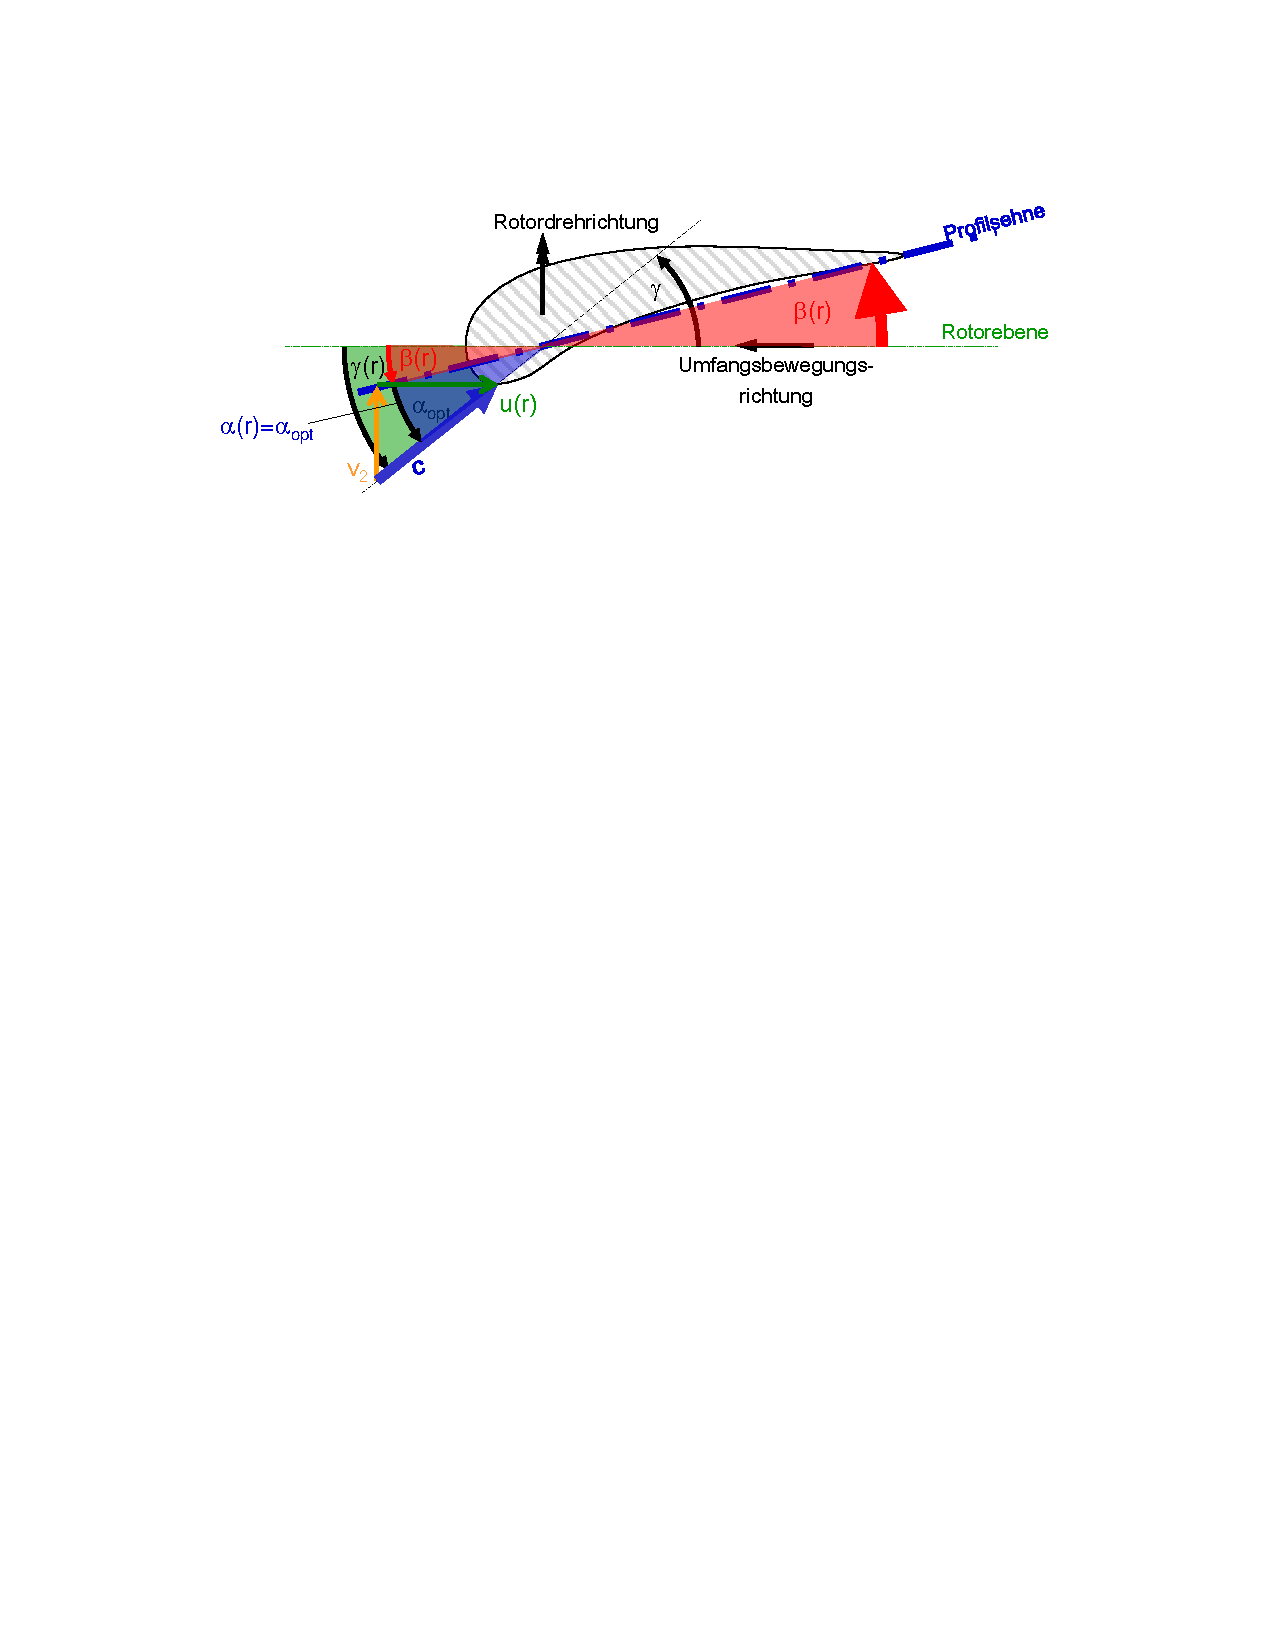
\includegraphics[width=0.6\textwidth]{Bilder/Kapitel 2/bauwinkel.pdf}}
   \caption[Bauwinkel]{Bauwinkel}
   \label{fig:Bild2.9}
\end{figure}

Da die Umfangsgeschwindigkeit bei gleichbleibenden Windverhältnissen von der Blattspitze bis zur Blattwurzel linear abnimmt und trotzdem ein optimale Anstellwinkel über die gesamte Blattlänge erreicht werden soll, muss das Rotorblatt verwunden werden. Andernfalls würde das Anströmverhältnis nicht im Optimum liegen. Der Bauwinkel nimmt zur Blattspitze hin ab. Die Blattkontur kann während des Betriebs nicht weiter verändert werden, folglich kann der Anstellwinkel nur noch durch die Anpassung der Rotordrehzahl, als auch durch das Verdrehen des gesamten Rotorblattes (Pitchen) verändert werden.

\paragraph{Wirkung der Auftriebs- und Widerstandskraft}\mbox{}\smallskip\\
Die Gleichungen zur Berechnung der Auftriebs- und Widerstandkraft beruhen auf \autoref{eq:Gleichung2.15} und \autoref{eq:Gleichung2.16}. Da die Anströmgeschwindigkeit $\acs{c}\left(\acs{R}, \acs{nR}\right)$ ebenfalls vom Anströmwinkel $\acs{gamma}\left(\acs{R}, \acs{nR}\right)$ abhängt, folgt:
\begin{align}
    \acs{FA}\left(\acs{alpha}\left(\acs{R}, \acs{nR}\right), \acs{gamma}\left(\acs{R}, \acs{nR}\right)\right) &= \acs{cA}\left(\acs{alpha}\left(\acs{R}, \acs{nR}\right)\right) \cdot \frac{1}{2} \cdot \acs{rho} \cdot \acs{c}\left(\acs{gamma}\left(\acs{R}, \acs{nR}\right)\right)^2 \cdot  \left(\acs{tflug} \cdot \acs{bflug}\right) \label{eq:Gleichung2.25} \\
    \acs{FW}\left(\acs{alpha}\left(\acs{R}, \acs{nR}\right), \acs{gamma}\left(\acs{R}, \acs{nR}\right)\right) &= \acs{cW}\left(\acs{alpha}\left(\acs{R}, \acs{nR}\right)\right) \cdot \frac{1}{2} \cdot \acs{rho} \cdot \acs{c}\left(\acs{gamma}\left(\acs{R}, \acs{nR}\right)\right)^2 \cdot \left(\acs{tflug} \cdot \acs{bflug}\right) \label{eq:Gleichung2.26}
\end{align}
\newline
Aus der Wurzel der quadratischen Addition von Auftriebs- und Widerstandskraft folgt eine resultierende Gesamtkraft $\acs{Fres}\left(\acs{alpha}, \acs{gamma}\right)$ (\autoref{eq:Gleichung2.27}), welche aus einer resultierenden Umfangskraft $\acs{deltaFU}\left(\acs{alpha}, \acs{gamma}\right)$ und einer Schubkraft $\acs{deltaFS}\left(\acs{alpha}, \acs{gamma}\right)$ besteht (\autoref{fig:Bild2.10}). Die resultierende Umfangskraft hat Biege- und Schubbelastungen von den Rotorblättern, Gondel, Turm und des Fundaments zur Folge. Hingegen erzeugt die Schubkaft eine Beschleunigung und Verzögerung der Rotordrehung.
\begin{equation}\label{eq:Gleichung2.27}
    \boxed{\acs{Fres}\left(\acs{alpha}, \acs{gamma}\right) = \sqrt{\acs{FA}\left(\acs{alpha}, \acs{gamma}\right)^2 + \acs{FW}\left(\acs{alpha}, \acs{gamma}\right)^2}}
\end{equation}
\begin{figure}[H]
   \centering
   \fbox{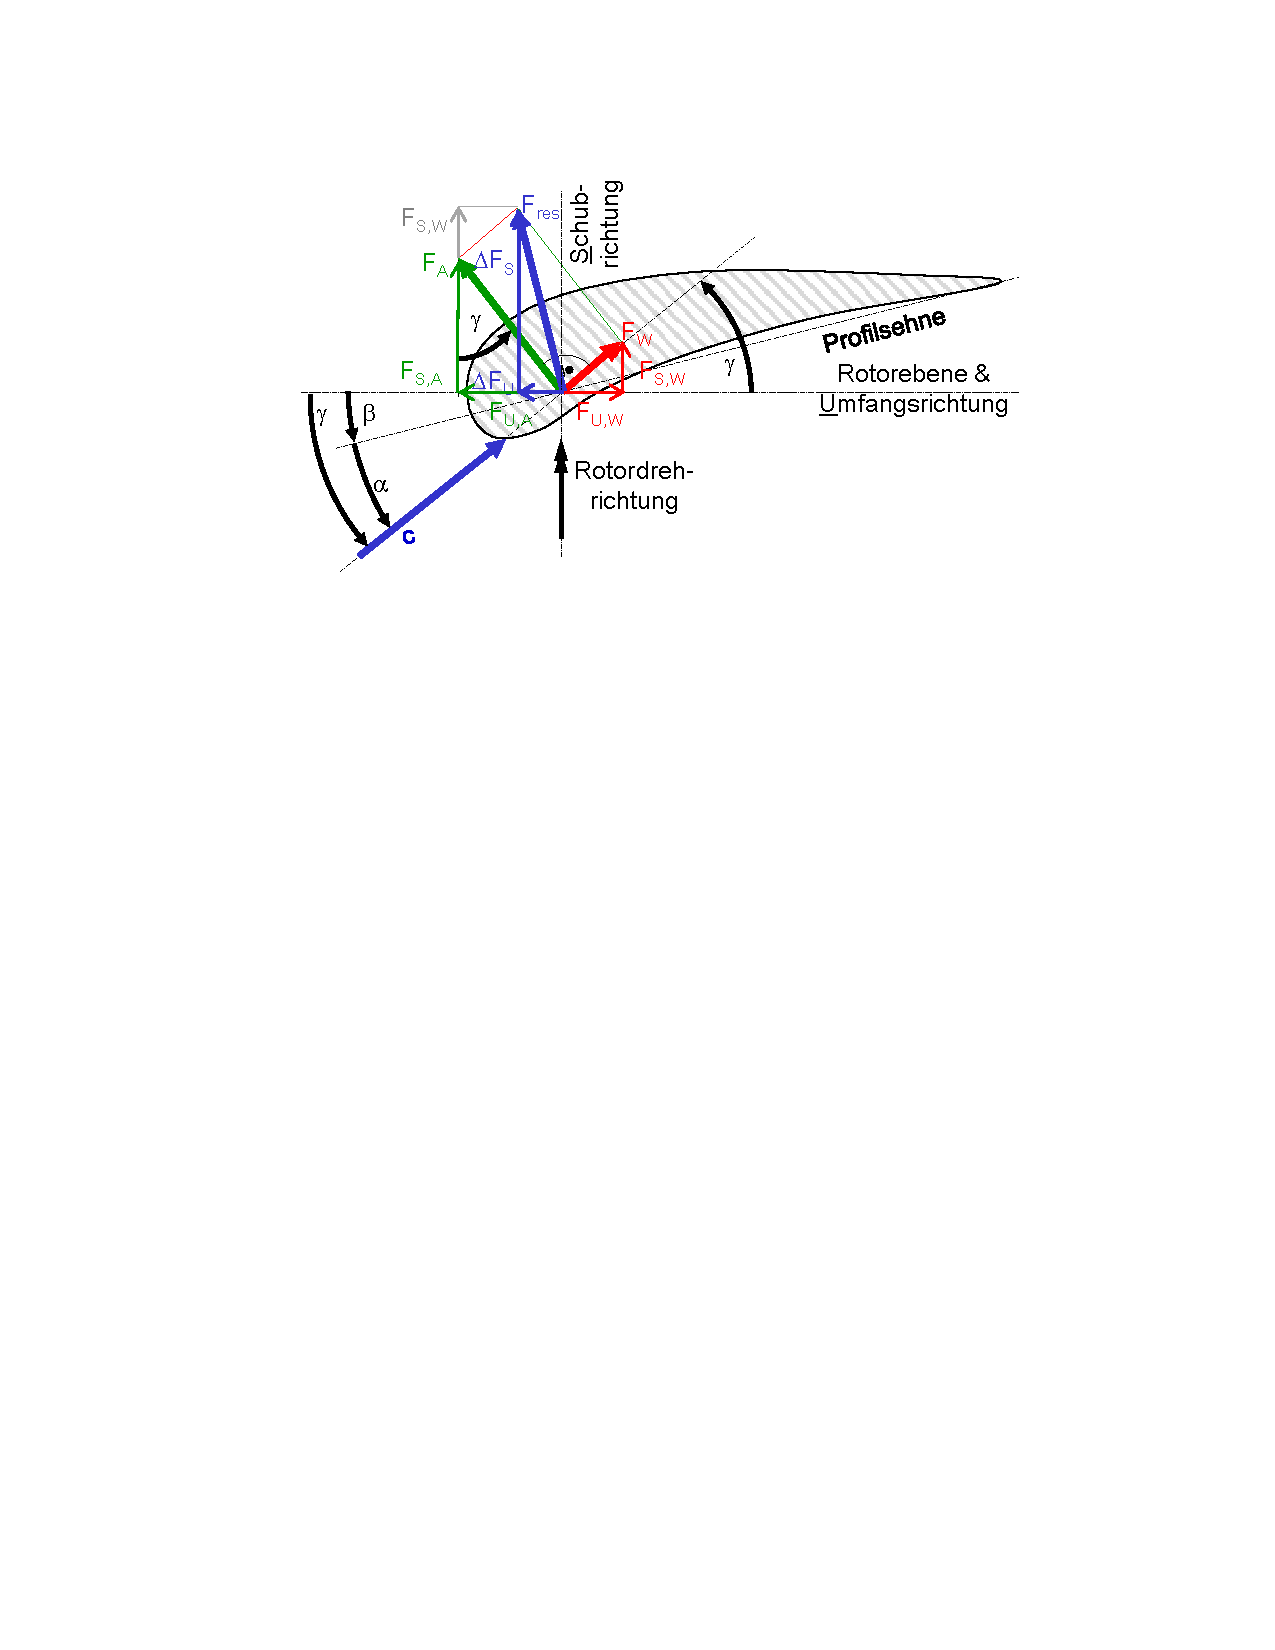
\includegraphics[width=0.6\textwidth]{Bilder/Kapitel 2/wirkung_auftriebs_widerstandskraft.pdf}}
   \caption[Wirkung der Auftriebs- und Widerstandskraft]{Wirkung der Auftriebs- und Widerstandskraft}
   \label{fig:Bild2.10}
\end{figure}

Die Kräfte $\acs{deltaFU}\left(\acs{alpha}, \acs{gamma}\right)$ und $\acs{deltaFS}\left(\acs{alpha}, \acs{gamma}\right)$ können aus den Längs- und Querkräften der Antriebs- und Widerstandskräften berechnet werden.
\begin{align*}
    \acs{FUA}\left(\acs{alpha}, \acs{gamma}\right) &= \acs{FA}\left(\acs{alpha}, \acs{gamma}\right) \cdot \sin(\acs{gamma}\left(\acs{R}, \acs{nR}\right))\\
    \acs{FUW}\left(\acs{alpha}, \acs{gamma}\right) &= \acs{FW}\left(\acs{alpha}, \acs{gamma}\right)\cdot \cos(\acs{gamma}\left(\acs{R}, \acs{nR}\right)) \\ 
    \acs{deltaFU}\left(\acs{alpha}, \acs{gamma}\right) &= \acs{FUA}\left(\acs{alpha}, \acs{gamma}\right) - \acs{FUW}\left(\acs{alpha}, \acs{gamma}\right)
\end{align*}
\begin{equation} \label{eq:Gleichung2.28}
    \boxed{\acs{deltaFU}\left(\acs{alpha}, \acs{gamma}\right) = \acs{FA}\left(\acs{alpha}, \acs{gamma}\right) \cdot \sin(\acs{gamma}\left(\acs{R}, \acs{nR}\right)) - \acs{FW}\left(\acs{alpha}, \acs{gamma}\right) \cdot \cos(\acs{gamma}\left(\acs{R}, \acs{nR}\right))}
\end{equation}
\smallskip
\begin{align*}
    \acs{FSA}\left(\acs{alpha}, \acs{gamma}\right) &= \acs{FA}\left(\acs{alpha}, \acs{gamma}\right) \cdot \cos(\acs{gamma}\left(\acs{R}, \acs{nR}\right))\\
    \acs{FSW}\left(\acs{alpha}, \acs{gamma}\right) &= \acs{FW}\left(\acs{alpha}, \acs{gamma}\right) \cdot \sin(\acs{gamma}\left(\acs{R}, \acs{nR}\right)) \\ 
    \acs{deltaFS}\left(\acs{alpha}, \acs{gamma}\right) &= \acs{FSA}\left(\acs{alpha}, \acs{gamma}\right) + \acs{FSW}\left(\acs{alpha}, \acs{gamma}\right)
\end{align*}
\begin{equation} \label{eq:Gleichung2.29}
    \boxed{\acs{deltaFS}\left(\acs{alpha}, \acs{gamma}\right) = \acs{FA}\left(\acs{alpha}, \acs{gamma}\right) \cdot \cos(\acs{gamma}\left(\acs{R}, \acs{nR}\right)) - \acs{FW}\left(\acs{alpha}, \acs{gamma}\right) \cdot \sin(\acs{gamma}\left(\acs{R}, \acs{nR}\right))}
\end{equation}
Die \autoref{eq:Gleichung2.28} und \autoref{eq:Gleichung2.29} gelten für ein Blattelement. Ein Rotorblatt besteht aus mehreren Blattelementen.

\subsubsection{Drehmomente und Leistungen}

\paragraph{Rotor- und Blattmoment}\mbox{}\smallskip\\
Das Rotordrehmoment \acs{MR} resultiert aus der Summation aller Teilmomente, welche aus dem Produkt von resultierender Umfangskraft \acs{deltaFU} und zugehöriger Radius resultieren. Da die WEA aus drei Rotorblättern besteht, wird die Summe zusätzlich mit dem Faktor drei multipliziert (\autoref{eq:Gleichung2.30}).
\begin{equation}\label{eq:Gleichung2.30}
    \boxed{\acs{MR}\left(\acs{R}, \acs{nR}\right) = 3 \cdot \sum_{i}^{} \acs{deltaFU}\left(\acs{ri}\right) \cdot \acs{ri}}
\end{equation}
\newline
Für das Blattmoment \acs{MB} kann die \autoref{eq:Gleichung2.30} als Referenz heranzgezogen werden. Die Umfangskraft wird lediglich durch die Schubkraft \acs{deltaFS} ersetzt (\autoref{eq:Gleichung2.31}).
\begin{equation}\label{eq:Gleichung2.31}
    \boxed{\acs{MB}\left(\acs{R}, \acs{nR}\right) = 3 \cdot \sum_{i}^{} \acs{deltaFS}\left(\acs{ri}\right) \cdot \acs{ri}}
\end{equation}

\paragraph{Rotorleistung}\mbox{}\smallskip\\
Durch die gewonnenen Erkenntnisse aus \autoref{eq:Gleichung2.30} über das Rotormoment \acs{MR} und mithilfe der Rotorwinkelgeschwindigkeit \acs{omegaR} kann nun eine Gleichung zur Berechnung der Rotorleistung berechnet werden, welche in direkter Abhängigkeit zur Rotordrehzahl \acs{nR} steht.
\begin{equation}
    \boxed{\acs{PR}\left(\acs{R}, \acs{nR}\right) = \left(3 \cdot \sum_{i}^{} \acs{deltaFS}\left(\acs{ri}\right) \cdot \acs{ri}\right) \cdot \acs{omegaR}\left(\acs{R}, \acs{nR}\right)}
\end{equation}
\newpage
\subsubsection{Leistungsanpassung}

\paragraph{Leistungsbegrenzung durch Pitchen}\mbox{}\smallskip\\
Beim Pitchen kann der Anstellwinkel \acs{alpha} durch das Drehen des gesamten Blattes um den Pitchwinkel \acs{ThetaP} an unterschiedliche Windgeschwindigkeiten \acs{v} angepasst werden. Der Anströmwinkel \acs{gamma} bleibt dabei unverändert.
\begin{figure}[H]
   \centering
   \fbox{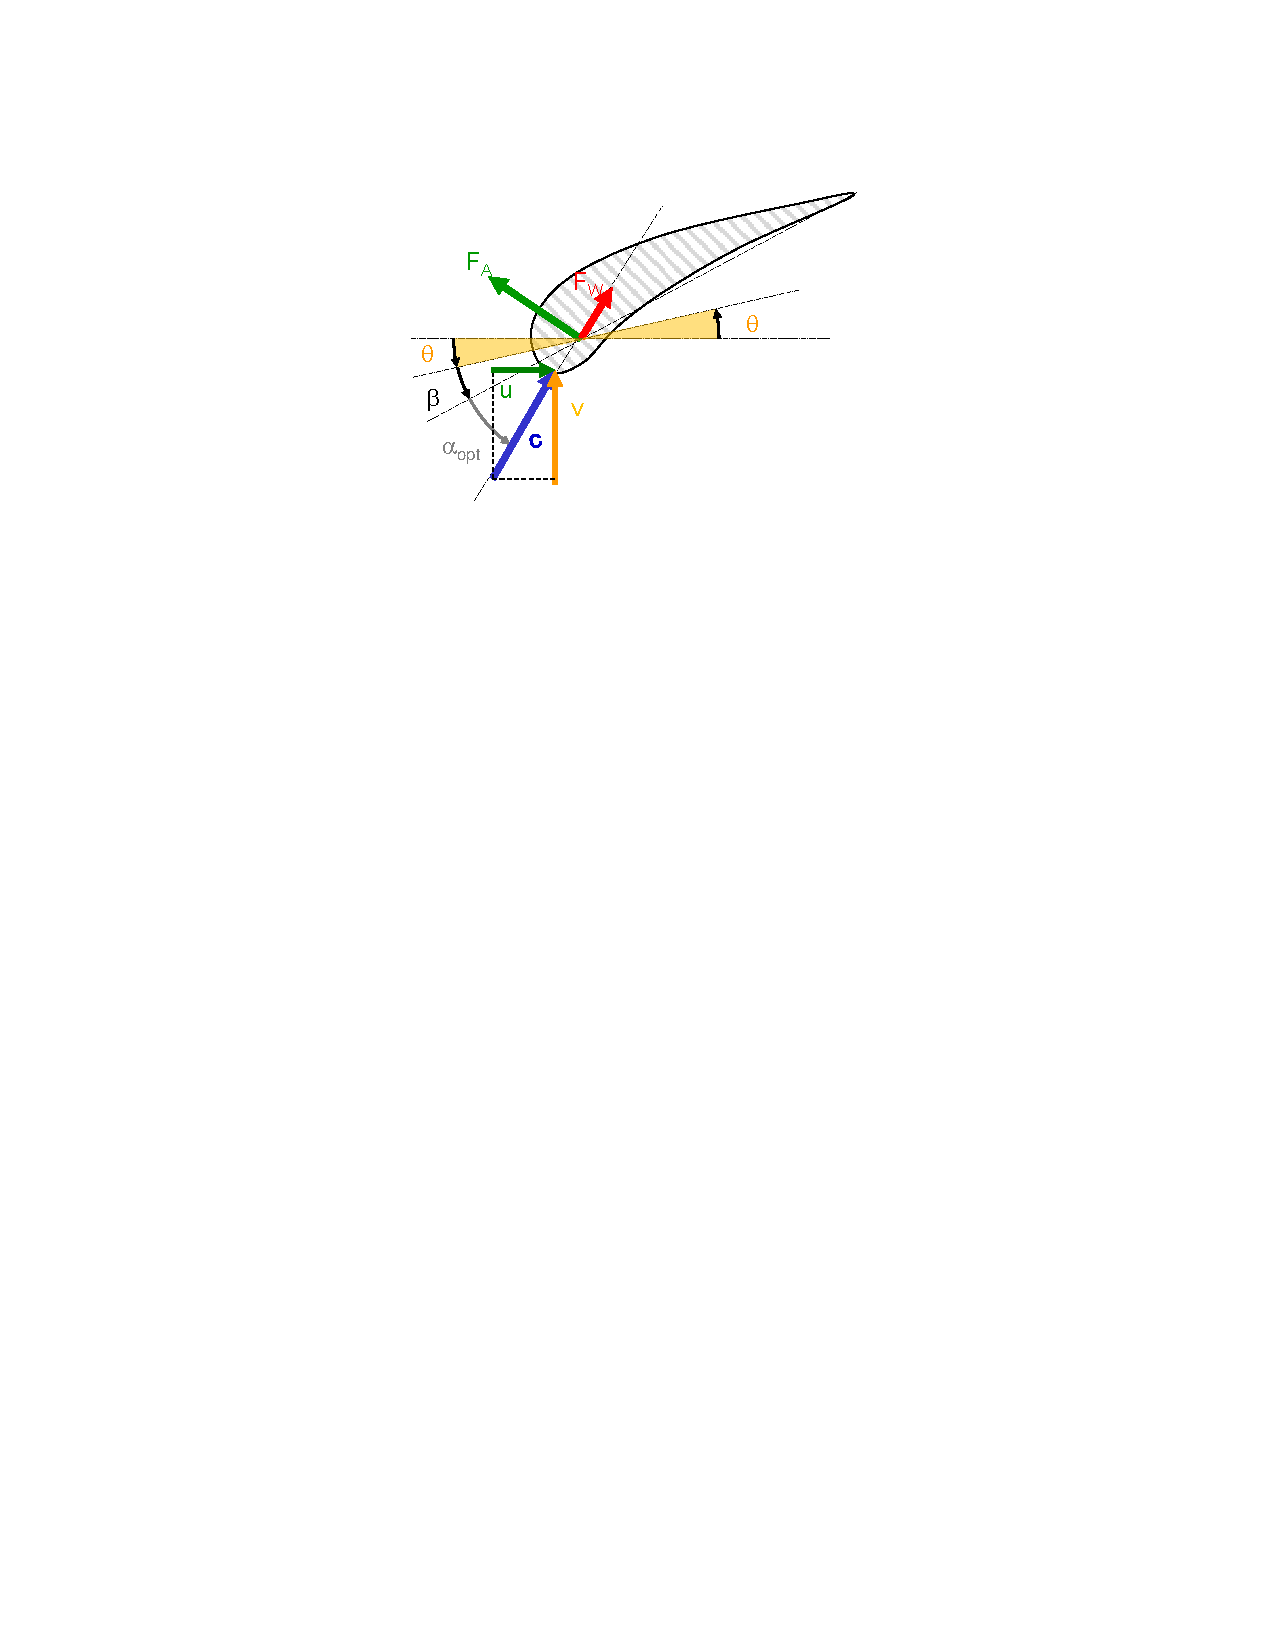
\includegraphics[width=0.5\textwidth]{Bilder/Kapitel 2/pitchen.pdf}}
   \caption[Pitchwinkel]{Pitchwinkel}
   \label{fig:Bild2.11}
\end{figure}

Da die Drehung jedoch eine langsame Stellgröße darstellt und die Windgeschwindigkeiten schnellen Änderungen unterliegen, ist das Pitchen lediglich zur Leistungsbegrenzung sinnvoll. Ein weiterer Nachteil ist, dass der optimale Anstellwinkel \acs{alphaopt} lediglich für ein Blattelement eingestellt wird, nicht aber für die gesamte Blattlänge.

\paragraph{Leistungsoptimierung durch Drehzahlanpassung}\mbox{}\smallskip\\
Als Alternative zum Pitchen, wird die Rotordrehzahl \acs{nR} und somit die Umfangsgeschwindigkeit \acs{u} entsprechend der Windgeschwindigkeiten in der Rotorebene nachgeführt, um ein optimales Anströmverhältnis und ein daraus resutlierenden optimalen Anstellwinkel \acs{alphaopt} zu garantieren. Der optimale Anstellwinkel hängt direkt vom Anströmwinkel ab, d.h. der Anstellwinkel ändert die Größe indirekt zur Rotordrehzahl. Durch die dynamische Drehzahlanpassung kann im Gegensatz zur Pitchwinkelverstellung der optimale Anstellwinkel für alle Blattelemente eingestellt werden.

\subsection{Zusammenführung von Stromröhren- und Tragflügeltheorie}
Die Grundlage der Zusammenführung bildet der Leistungsbeiwert \acs{cP}, welcher das Verhältnis von Rotorleistung \acs{PR} zu Windleistung \acs{PW} widerspiegelt (\autoref{eq:Gleichung2.13}).\\
Die Rotorleistung folgt dabei aus den Kenntnissen der Tragflügeltheorie in Abhängigkeit der resultierend Umfangskraft $\acs{deltaFU}\left(\acs{alpha}, \acs{gamma}\right)$ (\autoref{eq:Gleichung2.28}). Die Berechnung der zur Verfügung stehenden Windenergie resultiert aus der Stromröhrentheorie (\autoref{eq:Gleichung2.6}). Durch die Zusammenführung ist ein Zusammenhang zwischen Anstellwinkel \acs{alpha} und dem Leistungsbeiwert \acs{cP} hergestellt worden.

\subsubsection{Zusammenhang zwischen Anstellwinkel und Leistungsbeiwert}
Der Anstellwinkel \acs{alpha} bestimmt die Größe der Gleitzahl \acs{eps} (\autoref{eq:Gleichung2.18}), welche das Verhältnis von Antriebskraft $\acs{FA}\left(\acs{alpha}\right)$ zu Widerstandskraft $\acs{FW}\left(\acs{alpha}\right)$ bzw. der beiden Beiwerte $\acs{cA}\left(\acs{alpha}\right)$ und $\acs{cW}\left(\acs{alpha}\right)$ widergibt. Bei einem optimalen Anstellwinkel \acs{alphaopt} wird diese Verhältnis ebenfalls optimal und somit auch die Gleitzahl \acs{epsopt}.
\begin{equation*}
    \acs{alpha} \rightarrow \acs{alphaopt} \Rightarrow \acs{eps} \rightarrow \acs{epsopt}
\end{equation*}
\newline
Die resultierende Umfangskraft $\acs{deltaFU}\left(\acs{alpha}, \acs{gamma}\right)$ erreicht aufgrund der Abhängigkeit zu den Beiwerten ebenfalls das Optimum, wenn die Gleitzahl im Optimum ist.
\begin{equation*}
    \acs{epsopt} \Rightarrow \acs{deltaFU}_{\mathrm{opt}}
\end{equation*}
\newline
Da die notwendige Rotorleistung von der Umfangskraft abhängt, führt eine Steigerung der Umfangskraft \acs{deltaFU} zu einer einer Steigerung der Rotorleistung \acs{PR}.
\begin{equation*}
    \acs{deltaFU}\uparrow \Rightarrow \acs{PR}\uparrow
\end{equation*}
\newline
Durch den Anstieg der Rotorleistung, steigt das Verhältnis von Rotorleistung zu Windleistung und somit der Leistungsbeiwert \acs{cP}.
\begin{equation*}
    \acs{PR}\uparrow \Rightarrow \acs{cP}\uparrow
\end{equation*}
\newline
Somit wird geschlussfolgert, dass ein optimaler Anstellwinkel \acs{alphaopt} zu einem optimalen Leistungsbeiwert \acs{cPopt} führt. Da der Zusammenhang über die nicht monotone Funktion der Gleitzahl \acs{eps} hergestellt wurde, ist die Änderung des Leistungsbeiwertes \acs{cP} nicht proportional zu einer Änderung des Anstellwinkels \acs{alpha}.

\subsubsection{Momentenbeiwert}
Der Momentenbeiwert \acs{cM} wird als Quotient aus Leistungsbeiwert \acs{cP} und Schnellaufzahl \acs{lambda} definiert (\autoref{eq:Gleichung2.33}).
\begin{equation}\label{eq:Gleichung2.33}
    \boxed{\acs{cM} = \frac{\acs{cP}}{\acs{lambda}}}
\end{equation}
\newline
Aus den Kenntnissen über die Zusammenhänge von Leistungen und Momenten (\autoref{eq:Gleichung2.34} und \autoref{eq:Gleichung2.35}) folgt bei Gleichsetzung der Rotor- und Windleistung, dass der Momentenbeiwert ebenfalls den Quotienten aus Rotormoment \acs{MR} zu Windmoment \acs{MW} repräsentiert (\autoref{eq:Gleichung2.36}).
\begin{align}
    \acs{PW} &= \acs{MW} \cdot \acs{omegaR} \cdot \acs{cM} \label{eq:Gleichung2.34} \\
    \acs{PR} &= \acs{MR} \cdot \acs{omegaR} \label{eq:Gleichung2.35}
\end{align}
\begin{equation}\label{eq:Gleichung2.36}
    \boxed{\acs{cM} = \frac{\acs{MR}}{\acs{MW}}}
\end{equation}

\subsubsection{Zusammenfassung der Leistungen und Drehmomente von Rotor und Wind}
Das Winddrehmoment resultiert aus dem Produkt von Schukraft \acs{FST} und Blattradius \acs{R}. Zur Berechnung der Windleistung  gilt \autoref{eq:Gleichung2.7}.
\begin{align*}
    \acs{MW} = \acs{FST} \cdot \acs{R}
\end{align*}
\begin{equation}\label{eq:Gleichung2.37}
    \boxed{\acs{MW} = \frac{1}{2} \cdot \acs{rho} \cdot \acs{v1}^2 \cdot \acs{A2} \cdot \acs{R}}
\end{equation}
\newline
\begin{align*}
    \acs{PW} = \acs{FST} \cdot \acs{v1}
\end{align*}
\begin{equation}\label{eq:Gleichung2.38}
    \boxed{\acs{PW} = \frac{1}{2} \cdot \acs{rho} \cdot \acs{v1}^3 \cdot \acs{A2}}
\end{equation}
\newline
Die Gleichungen zur Berechnung des Rotordrehmoments \acs{MR} und der Rotorleistung \acs{PR} ruhen auf Basis von \autoref{eq:Gleichung2.12} und \autoref{eq:Gleichung2.36}.
\begin{align*}
    \acs{MR} = \acs{FST} \cdot \acs{R} \cdot \acs{cM}
\end{align*}
\begin{equation}\label{eq:Gleichung2.39}
    \boxed{\acs{MR} = \frac{1}{2} \cdot \acs{rho} \cdot \acs{v1}^2 \cdot \acs{A2} \cdot \acs{R} \cdot \acs{cM}}
\end{equation}
\newline
\begin{align*}
    \acs{PR} = \acs{FST} \cdot \acs{v1} \cdot \acs{cP}
\end{align*}
\begin{equation}\label{eq:Gleichung2.40}
    \boxed{\acs{PR} = \frac{1}{2} \cdot \acs{rho} \cdot \acs{v1}^2 \cdot \acs{A2} \cdot \acs{v1} \cdot \acs{cP}}
\end{equation}

\subsection{WEA-Kennfelder}

\subsection{Lookup Tables}
